\documentclass[../main.tex]{subfiles}

\begin{document}

\chapter{代码主体结构}
\vspace{-2cm}

简要总结

\section{整体框架}

- 参考 \url{https://github.com/XPixelGroup/BasicSR/blob/master/docs/DesignConvention_CN.md}

- 代码接口在 http://basicsr.readthedocs.io/,后续看看能否作为附录存在

%##################################################################################################
\begin{figure}[t]
    %\vspace{-0.5cm}
    \begin{center}
        %\fbox{\rule{0pt}{2.5in} \rule{0.9\linewidth}{0pt}}
        
\includegraphics[width=\linewidth]{figures/basicsr_logo.png}
        \vspace{-1cm}
        \caption{图标题。BasicSR Logo。}
        \label{fig:logo}
    \end{center}
    %\vspace{-0.7cm}
\end{figure}
%##################################################################################################

\section{配置(Options)与注册器(Register)}\label{Register}

- 态实例化与REGISTER注册机制

- 约定

- 如何避免重复的类名和函数名

% \begin{minted}[xleftmargin=20pt,linenos,bgcolor=bg,breaklines]{python}
% class RepConv(nn.Module):
%     """Re-parameterizable block for RepSR."""

%     def ___init___(self,
%                  in_channels,
%                  out_channels,
%                  kernel_size,
%                  stride=1,
%                  padding=0,
%                  dilation=1,
%                  groups=1,
%                  padding_mode='zeros',
%                  deploy=False,
%                  width_multiplier=2,
%                  with_bn=True,
%                  frozen_bn=False):
%         super(RepConv, self).___init___()
%         self.deploy = deploy
%         self.in_channels = in_channels
%         self.out_channels = out_channels
%         self.kernel_size = kernel_size
%         self.stride = stride
%         self.padding = padding
%         self.dilation = dilation
%         self.groups = groups
%         self.with_bn = with_bn
%         self.frozen_bn = frozen_bn

%         self.mid_channels = out_channels * width_multiplier
%         self.rep_c1_2 = nn.Conv2d(
%             in_channels=self.mid_channels,
%             out_channels=out_channels,
%             kernel_size=1,
%             stride=stride,
%             padding=0,
%             groups=groups,
%             bias=True)

%         # initialization
%         init_list = [
%             self.rep_identity, self.rep_c3_1, self.rep_c1_1, self.rep_c3_2,
%             self.rep_c1_2
%         ]
%         if with_bn:
%             init_list.extend([self.rep_bn_1, self.rep_bn_2])
%         default__init__weights(init_list, scale=0.1)

%     def forward(self, inputs, frozen_bn=None):
%         if frozen_bn is None:
%             frozen_bn = self.frozen_bn

%         if hasattr(self, 'rep_merge'):
%             return self.rep_merge(inputs)
%         if self.with_bn:
%             id_out = self.rep_identity(inputs)
%             out_1 = self.rep_c1_1(
%                 self.rep_bn_1(self.rep_c3_1(inputs), frozen_bn))
%             out_2 = self.rep_c1_2(
%                 self.rep_bn_2(self.rep_c3_2(inputs), frozen_bn))
%         else:
%             id_out = self.rep_identity(inputs)
%             out_1 = self.rep_c1_1(self.rep_c3_1(inputs))
%             out_2 = self.rep_c1_2(self.rep_c3_2(inputs))

%         return id_out + out_1 + out_2
% \end{minted}


\section{数据(Data Loader)}

\section{网络结构(Architecture)}


本文档旨在完整地介绍 BasicSR 的设计和框架,为入门者提供一份上手指南,为使用者提供一份日常参考。

本文档不涉及具体函数和代码的介绍。如果需要具体函数和代码的介绍,请查阅 BasicSR 的在线 API 文档。我们更推荐读者直接查看代码,这样可以更加完整、细致的了解实现细节。

\begin{hl} % ---------------- Highlight block ---------------- %
	\textbf{BasicSR API 文档}

	BasicSR 的 API 文档是实时更新的,并且发布在 readthedocs.io 网站上:

	\url{https://basicsr.readthedocs.io/en/latest/}

	国内可能访问速度缓慢,后续我们会考虑导出 PDF 文档作为附录。
\end{hl}

\section{模型 (Model)}

模型部分定义了许多模型级别的操作,比如训练设置、训练数据如何送入模型、优化器的选择、损失函数计算、模型参数更新、训练中验证、测试过程等。模型部分定义在:
\dirtree{%
	.1 ROOT\_DIR.
	.2 BasicSR.
	.3 basicsr.
	.4 models.
	.5 \_\_init\_\_.py.\DTcomment{扫描所有models并注册,实例化某模型}.
	.5 base\_model.py\DTcomment{模型的基类,定义许多共同操作}.
	.5 edvr\_model.py.
	.5 esrgan\_model.py.
	.5 hifacegan\_model.py.
	.5 realesrgan\_model.py.
	.5 realesrnet\_model.py.
	.5 sr\_model.py\DTcomment{图像超分模型}.
	.5 srgan\_model.py.
	.5 stylegan2\_model.py.
	.5 swinir\_model.py.
	.5 video\_base\_model.py\DTcomment{视频超分基类模型}.
	.5 video\_gan\_model.py.
	.5 video\_recurrent\_gan\_model.py.
	.5 video\_recurrent\_model.py.
}

其中 \_\_init\_\_.py 会自动扫描 basicsr/models 中的文件,如果是以 \_model.py 结尾的,则为其中注册器中的模型进行 import 。然后根据 option 中的 model\_type 实例化对应模型并返回。

\begin{note} % ---------------- Note block ---------------- %
	注册器参见章节\ref{Register}。
\end{note}

为增加模型间的复用, 我们大量使用了继承, 以下为各个模型之间的继承关系:

\dirtree{%
	.1 Base\_Model.
	.2 SR\_Model.
	.3 SRGAN\_Model.
	.4 ESRGAN\_Model.
	.4 RealESRGAN\_Model.
	.3 RealESRNet\_Model.
	.3 SwinIR\_Model.
	.3 Video\_Base\_Model.
	.4 EDVR\_Model.
	.4 VideoRecurrent\_Model.
	.5 VideoRecurrentGAN\_Model.
	.3 HiFaceGAN\_Model.
	.2 StyleGAN2\_Model.
}

下面具体介绍一些重要模型及其功能,以及如何按照自己的需求自定义新的模型。

\subsection{Base Model}
Base Model是所有模型的基类,定义一些共同操作。比如:

代码位置:\href{https://github.com/XPixelGroup/BasicSR/blob/master/basicsr/models/base_model.py}{BasicSR/basicsr/models/base\_model.py}
\begin{minted}[xleftmargin=20pt,breaklines,linenos,bgcolor=bg]{python}

def print_network(self, net):
# 输出网络信息

def save_network(self, net, net_label, current_iter, param_key='params'):
# 保存模型

def save_training_state(self, epoch, current_iter):
# 保存训练状态

def load_network(self, net, load_path, strict=True, param_key='params'):
# 加载模型

def get_optimizer(self, optim_type, params, lr, **kwargs):
# 定义优化器

def _get__init__lr(self):
# 定义初始学习率

def update_learning_rate(self, current_iter, warmup_iter=-1):
# 学习率更新

def setup_schedulers(self):
# 学习率调度器
\end{minted}

\begin{hl} % ---------------- Highlight block ---------------- %
Base Model 的很多函数,可以在继承后的模型中根据要求来重写,比如不同模型读取数据的方式不同,则会重写不同的 feed\_data() 函数。
\end{hl}

\subsection{其他模型,以 SR Model 为例}\label{Model:SR Model}

SR Model 是图像超分辨率模型的类,定义了基础的单张图像超分辨率模型。下面从一个模型的训练角度展示其中重要的函数:

代码位置:\href{https://github.com/XPixelGroup/BasicSR/blob/master/basicsr/models/sr_model.py}{BasicSR/basicsr/models/sr\_model.py}

\begin{minted}[xleftmargin=20pt,linenos,bgcolor=bg,breaklines]{python}

class SRModel(BaseModel):
    """Base SR model for single image super-resolution."""

    def ___init___(self, opt):
        
    def init_training_settings(self):
    # 初始化训练设置。包括优化器、损失函数的定义,学习率的初始化等。
    
    def setup_optimizers(self):
    # 设置优化器,可以控制哪些参数会被更新。详情参阅4.7优化器部分。
       
    def feed_data(self, data):
    # 把训练数据送入模型。这里是从 dataloader 中取出数据,用于训练或测试。在 SR Model 中,每次取用一个 batch(n,c,h,w) 数量的 LR 和 GT 图像。

    # 其他模型对batch做不同操作时,经常会改写这个函数。比如只读取 GT 、读取额外 label 、读取图像路径、对读取的数据增加 degradation 等操作,都通过修改 feed\_data() 来实现。
       
    def optimize_parameters(self, current_iter):
    # 更新模型参数。在这个函数中,会实际调用模型跑出 SR 图像,再将 SR 与 GT 代入损失函数计算 loss,并且进行 loss 的回传和参数的更新。当有多个 loss 或需要自己添加 loss 时,或者需要特殊的更新步骤时,修改这里。
   
    # 比如在 GAN 系列的 Model 中,这个函数就是 SR 图像与 GT 一起输入判别网络来得到 loss ,再将不同的 loss 进行加权组合。并且 Generator 和 Discriminator 的参数都需要更新。

    def nondist_validation(self, dataloader, current_iter, ...):
    # 训练中进行验证。会停止训练,调用 test() ,进行验证并记录指标、保存结果图,然后继续训练。

    def get_current_visuals(self):
    # 将当前图片从 GPU 中取出,以进行保存或其它操作。
        
    def save(self, epoch, current_iter):
    # 保存模型。
\end{minted}

其他model的思想与SR Model大同小异,都是相互继承公用的函数,单独改写有特别需求的函数,完成一个模型包括获得数据、更新参数、验证等步骤的训练过程。


\subsection{自定义模型,以 SRGAN Model 为例}

当需要自定义某个模型的时候,首先在 \href{https://github.com/XPixelGroup/BasicSR/blob/master/basicsr/models}{BasicSR/basicsr/models} 下新建 XXX\_model.py 文件,根据需要写一个新类(注意不要与现有类重名)继承 Base Model 或其他 model ,然后根据自己的需求改写主要函数即可。

比如 SRGAN\_Model 继承了绝大多数 SR\_Model 的函数,但是改写了 optimize\_parameters() ,适应 GAN 的参数更新需要。而 RealSRGAN\_Model 又继承了 SRGAN\_Model ,改写了 feed\_data() 以在线生成带有不同 degradation 的训练数据。

\begin{note} % ---------------- Note block ---------------- %
	上述被改写函数的介绍,参见章节\ref{Model:SR Model}。
\end{note}

\section{损失函数 (Loss)}

损失函数部分定义了很多常用的损失函数。损失函数部分定义在:
\dirtree{%
	.1 ROOT\_DIR.
	.2 BasicSR.
	.3 basicsr.
	.4 losses.
	.5 \_\_init\_\_.py.\DTcomment{扫描所有 loss 并注册,实例化某些损失函数}.
	.5 losses.py.\DTcomment{损失函数的具体实现}.
	.5 loss\_util.py.\DTcomment{损失函数工具,如对损失函数加权、累加、平均等}.
}
\subsection{损失函数的使用}

损失函数主要在不同 model 里被定义、计算和使用。下面是一个例子。

代码位置:\href{https://github.com/XPixelGroup/BasicSR/blob/master/basicsr/models/sr_model.py}{BasicSR/basicsr/models/sr\_model.py},其他 model 文件中也有。

\begin{minted}[xleftmargin=20pt,linenos,bgcolor=bg,breaklines]{python}

def init_training_settings(self):
    ……
    self.cri_pix = build_loss(train_opt['pixel_opt']).to(self.device)
    # 定义损失函数


def optimize_parameters(self, current_iter):
    self.optimizer_g.zero_grad()
    # 优化器梯度归零

    l_pix = self.cri_pix(self.output, self.gt)
    # 在更新参数时,需要计算 loss
    l_total += l_pix
    loss_dict['l_pix'] = l_pix
    # 将 loss 记录到 log 文件里
    
    l_total.backward()
    # loss 反向传播,计算梯度
    
    self.optimizer_g.step()
    # 更新网络参数
\end{minted}

\subsection{自定义损失函数}

在 \href{https://github.com/XPixelGroup/BasicSR/blob/master/basicsr/losses/losses.py}{BasicSR/basicsr/losses/losses.py} 下写一个新的损失函数类,并将类名写入\href{https://github.com/XPixelGroup/BasicSR/blob/master/basicsr/losses/__init__.py}{BasicSR/basicsr/losses/\_\_init\_\_.py}。可以参考其他损失函数类的写法,对一个 batch 的数据进行计算并返回 loss 的值。

\section{训练[优化器 (optimizer) 与学习率调度器 (scheduler) ]}

\begin{note} % ---------------- Note block ---------------- %
	训练的整体pipeline参见\ref{}。
\end{note}

本节主要介绍其中的优化器、优化步骤和学习率调度相关内容。当训练进行到更新模型参数时,即
\begin{minted}[xleftmargin=20pt,linenos,bgcolor=bg,breaklines]{python}
model.optimize_parameters(current_iter) # 在BasicSR/basicsr/train.py
\end{minted}

模型会运行得到结果、计算loss并根据优化器进行参数优化,然后更新学习率。

这个步骤的具体代码定义在BasicSR/basicsr/models中具体的Model里,因为需要计算的loss的步骤是各不相同的,比如GAN需要经过判别器。

代码位置:\href{https://github.com/XPixelGroup/BasicSR/blob/master/basicsr/models/sr_model.py}{BasicSR/basicsr/models/sr\_model.py},其他 model 文件中也有。

\begin{minted}[xleftmargin=20pt,linenos,bgcolor=bg,breaklines]{python}

def optimize_parameters(self, current_iter):
    self.optimizer_g.zero_grad()
    # 优化器梯度归零

    # 计算loss,代码省略
    
    l_total.backward()
    # loss反向传播,计算梯度
    
    self.optimizer_g.step()
    # 更新网络参数
\end{minted}

此时,optimizer 就会去更新参数。 optimizer 在 init\_training\_setting 中定义,定义的时候,会定义好哪些参数需要更新、按照什么样的方法去更新(优化方法)。

代码位置:\href{https://github.com/XPixelGroup/BasicSR/blob/master/basicsr/models/sr_model.py}{BasicSR/basicsr/models/sr\_model.py},其他 model 文件中也有。

\begin{minted}[xleftmargin=20pt,linenos,bgcolor=bg,breaklines]{python}

def setup_optimizers(self):
    train_opt = self.opt['train']
    optim_params = []
    for k, v in self.net_g.named_parameters():
        # 对于网络中的所有需要梯度的参数,添加进优化器中。
        # 这里可以按照结构名称,来规定哪些参数需要使用当前优化器更新。
        if v.requires_grad:
            optim_params.append(v)
        else:
            logger = get_root_logger()
            logger.warning(f'Params {k} will not be optimized.')

    optim_type = train_opt['optim_g'].pop('type')
    # 这里定义优化器的优化方法,如Adam
    self.optimizer_g = self.get_optimizer(...)
    self.optimizers.append(self.optimizer_g)
    # 把当前这个优化器放到optimizers里面,也就是说可以定义多个优化器去优化同一网络的不同参数部分。
\end{minted}

而优化器更新参数时的学习率,来源于学习率调度器 scheduler。 scheduler 同样在 init\_training\_setting 中定义。学习率更新时,就是调用 scheduler ,来生成当前需要的学习率。代码在 \href{https://github.com/XPixelGroup/BasicSR/blob/master/basicsr/models/base_model.py}{BasicSR/basicsr/models/base\_model.py} 中:

\begin{minted}[xleftmargin=20pt,linenos,bgcolor=bg,breaklines]{python}

def setup_schedulers(self):
    # 选择scheduler类型,比如训练多少次迭代后,学习率衰减(MultiStepLR)。
\end{minted}



\section{算子 (Operator)}

\subsection{什么是算子?}

当使用pytorch时,绝大多数操作为张量 (Tensor) 的运算。张量计算的种类有很多,比如加法、乘法、矩阵相乘、矩阵转置等,这些计算被称为算子 (Operator),它们是PyTorch的核心组件。

一般情况下,pytorch推荐使用python层的前端语言来构建新的算子。但是有时候出于一些其他方面的考虑,会需要增加底层算子。例如有时候对性能要求很高,python不满足需求,又或者是需要链接其他的动态库(blas,mkl等),因此pytorch也提供了直接扩展底层C++算子的能力。

\subsection{BasicSR 中的自定义算子}

BasicSR中所用的自定义算子代码在 \href{https://github.com/XPixelGroup/BasicSR/tree/master/basicsr/ops}{BasicSR/basicsr/ops} 中。采用C++ extension的方式添加。它与pytorch的相互解耦,分开编译,所以增加算子不需要修改pytorh的源码。它的原理其实就是通过pybind11,将C++编译为pytroch的一个模块,这样就可以在pytorch中通过这个新的模块来执行新的操作了。添加方法详情参阅 \href{https://pytorch.org/tutorials/advanced/cpp_extension.html#writing-a-mixed-c-cuda-extension}{pytorch官方文档} 。

BasicSR中的自定义算子主要有deform\_conv,upfirdn2d,fused\_act三大类。deform\_conv主要用在各个视频恢复的模型上,是一种隐式的对齐方式。upfirdn2d,fused\_act,用在stylegan2中。

\subsection{BasicSR 中算子的编译、安装、使用}

\begin{note} % ---------------- Note block ---------------- %
	编译和安装的过程参见\ref{Register}。
\end{note}

当算子成功编译之后,调用自定义算子就像调用pytorch原生算子一样。


\begin{minted}[xleftmargin=20pt,linenos,bgcolor=bg,breaklines]{python}
# 调用pytorch原生算子
from torch import nn

Class xxx():
    def __init__():
        conv1 = nn.Conv2d(……)

    def forward():
        out = conv1(……)

# 调用自定义算子,可以直接在forward中使用
from basicsr.ops.upfirdn2d import upfirdn2d
    
    def forward():
        out = upfirdn2d(……)

\end{minted}


\section{日志系统 (Logger)}

BasicSR 的日志系统主要包括实验过程中1.记录的 log 文件和2.可以通过 tensorboard 可视化的 tb\_logger。

日志系统的实现不过多赘述,如果有兴趣可以参阅 \href{https://github.com/XPixelGroup/BasicSR/blob/master/basicsr/utils/logger.py}{BasicSR/basicsr/utils/logger.py}。本章节主要讲述日志系统各个项目代表什么;以及如何改代码,在日志中记录我们想记录的个性化内容。

\subsection{log 文件记录及解读}

当进行实验的时候,代码会在 BasicSR/experiments 中创建一个属于当前实验的文件夹,文件夹名字为实验名,文件夹中会存在一个 log 文件,下面我们来说明如何按照我们自己的要求记录 log 文件,以及现有 log 文件每个条目的意义。

\begin{hl} % ---------------- Highlight block ---------------- %

添加一条 log 信息非常简单:

\begin{minted}[xleftmargin=20pt,linenos,bgcolor=bg,breaklines]{python}
logger.info(要添加的内容) # 添加正常信息
logger.warning(要添加的警告) # 添加警告信息
\end{minted}
\end{hl}

在 model 文件中,已经定义好 logger 的情况下,只要在合适的位置添加上述语句,即可记录信息。每个 model 文件中都有大量的 logger 添加,故不具体展示使用位置,有兴趣的读者可以自己在 model 文件中搜索。

下面是一个 log 文件的例子:

\begin{minted}[xleftmargin=20pt,linenos,bgcolor=bg,breaklines]{python}
# BasicSR/basicsr/experiments/实验名字/xxxx.log
2022-06-17 02:27:36,068 INFO: 
# 在代码中调用logger.info(要添加的内容)后,会自动记录时间并增加条目 INFO:下面log中我删掉了时间信息,节省篇幅

Version Information: 
# 软件的版本
	BasicSR: 1.3.3.10
	PyTorch: 1.9.1+cu111
	TorchVision: 0.10.1+cu111
INFO: 
  name: 000_SRResNet_DIV2K
  # 实验名,整个options的内容都会记录在这里,本文件中省略掉了。
  

INFO: Dataset [XXXDataset] - XXXdata is built.
INFO: Training statistics:
# 训练数据的信息,数量、batchsize等
	Number of train images: 38684
	Dataset enlarge ratio: 1
	Batch size per gpu: 16
	World size (gpu number): 1
	Require iter number per epoch: 2418
	Total epochs: 207; iters: 500000.
INFO: Dataset [PairedImageDataset] - validation is built.
# dataset类型
INFO: Number of val images/folders in validation: 14
# 验证集信息
INFO: Network [MSRResNet] is created.
INFO: Network: MSRResNet, with parameters: 1,222,147
# 网络参数量
INFO: MSRResNet(
# 网络结构,此处省略
  
INFO: Use Exponential Moving Average with decay: 0.999
INFO: Loss [L1Loss] is created.
INFO: Model [RealESRNetModel_XXX] is created.
INFO: Start training from epoch: 0, iter: 0
# 开始训练
INFO: [XXX_0..][epoch:  0, iter:     100, lr:(2.000e-04,)] [eta: 2 days, 21:55:41, time (data): 0.040 (0.004)] l_pix: 5.0581e-02 
# epoch:第几轮;iter:第几次迭代(一次迭代是一个batch), lr:学习率][eta:剩余时间预估 time (data):跑了百分之多少的数据了] l_pix:当前的loss 
INFO: Validation validation
# 验证集验证结果
	 #  psnr: 18.0289
	 
INFO: End of training. Time consumed: 10:22:17
INFO: Save the latest model.
INFO: Validation validation
# 训练结束,最终验证集结果
	 #  psnr: 20.7466
	 
\end{minted}

\subsection{tb\_logger 记录及解读}

除了上述的 log 文件外,BasicSR 还会生成可以用 tensorboard 打开的 tb\_logger 文件。一般保存在 BasicSR/experiments/tb\_logger/ 实验名。


开启: 在 yml 配置文件中设置 `use\_tb\_logger: true`:
\begin{minted}[xleftmargin=20pt,linenos,bgcolor=bg,breaklines]{python}
# yml
    logger:
      use_tb_logger: true
\end{minted}

在浏览器中查看:
\begin{minted}[xleftmargin=20pt,linenos,bgcolor=bg,breaklines]{python}
# bash
    tensorboard --logdir tb_logger --port 5500 --bind_all
\end{minted}

\begin{figure}[h]
    %\vspace{-0.5cm}
    \begin{center}
        %\fbox{\rule{0pt}{2.5in} \rule{0.9\linewidth}{0pt}}
        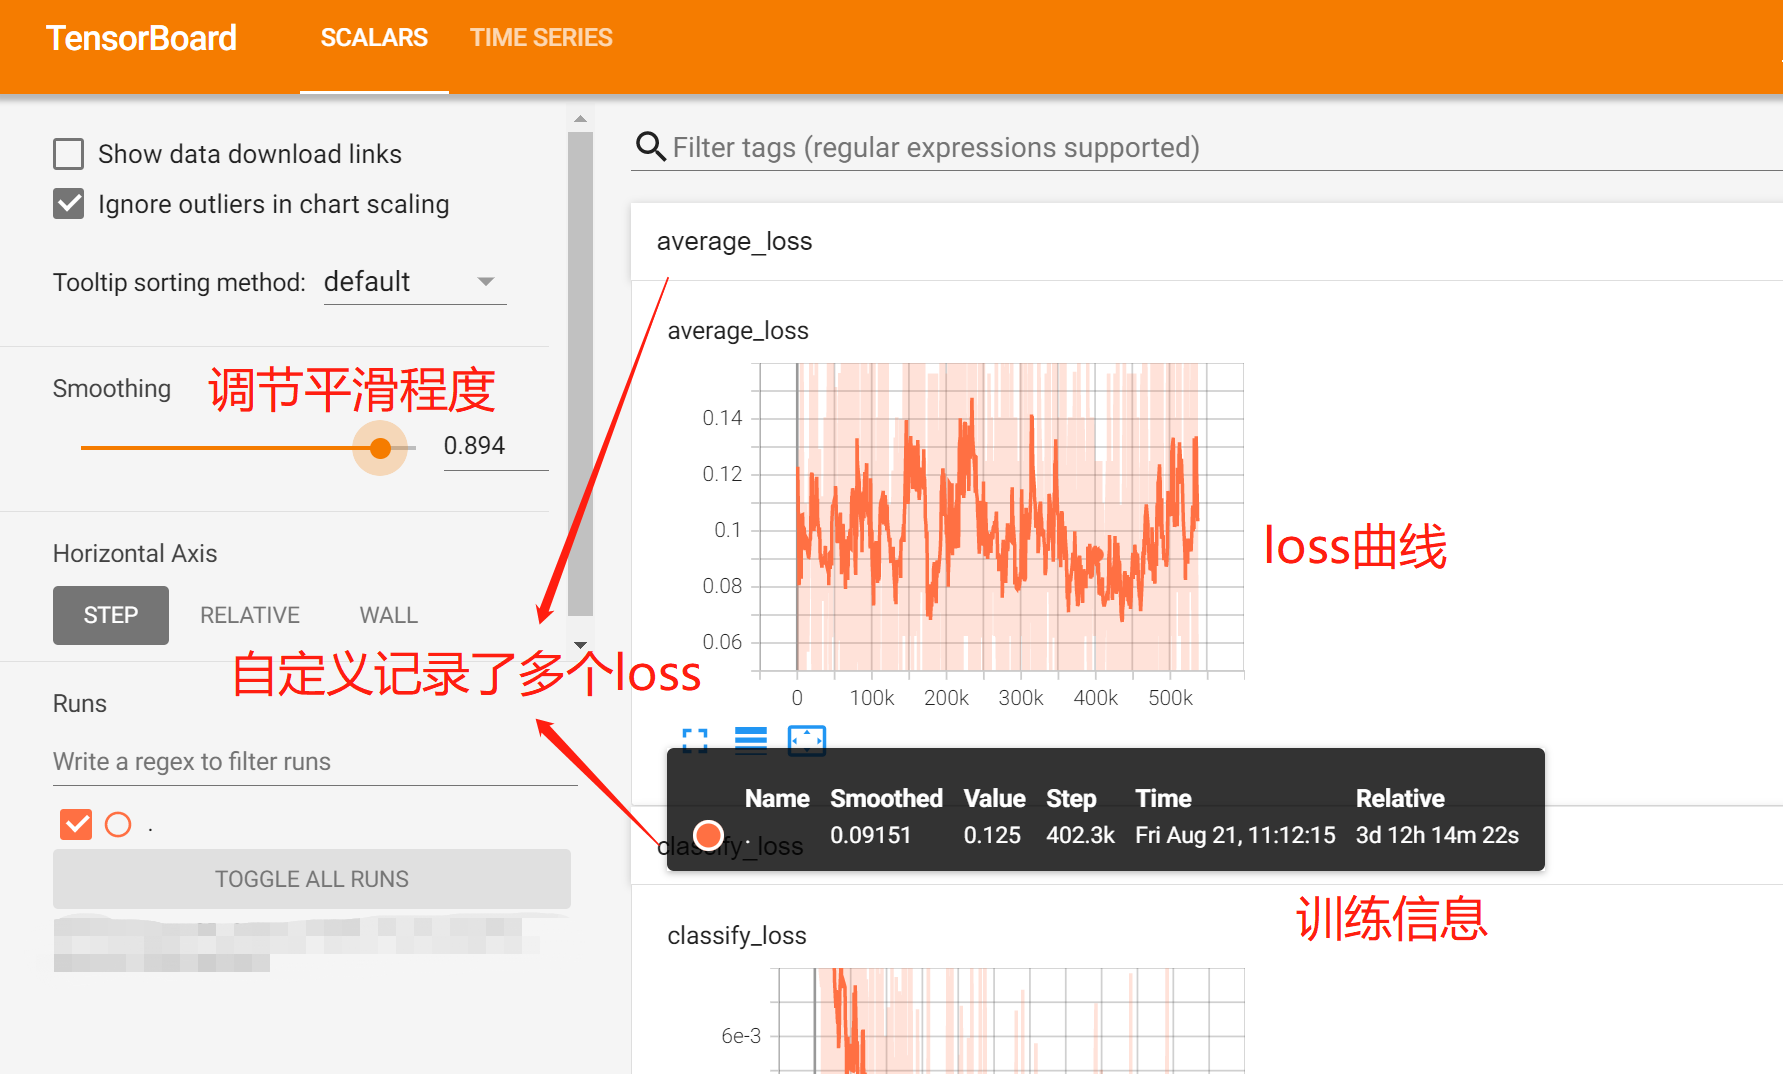
\includegraphics[width=0.8\linewidth]{figures/tensorboard_demo.png}
        % \vspace{-1cm}
        \caption{tensorboard示例图}
        \label{fig:tensorboard_demo}
    \end{center}
    %\vspace{-0.7cm}
\end{figure}

目前 BasicSR 里 tb\_logger 主要记录 validation 结果和训练过程中的 loss。validation 结果会随增加 metric 而增加,不过多赘述,重点介绍如何添加 loss 记录到 tb\_logger 。

\begin{hl} % ---------------- Highlight block ---------------- %
虽说封装的很深,但是实际在框架中使用起来,只需要在 xx\_model.py 计算 loss 之后,把新的 loss, loss\_dict['新的loss'] = 新的loss ,即可同时记录在 tb\_logger 和 los 文件中。
也可以使用这种方法记录不是 loss 的其他值。
\end{hl}

下面介绍具体的封装细节,tb\_logger 的初始化和记录代码为:

\begin{minted}[xleftmargin=20pt,linenos,bgcolor=bg,breaklines]{python}
tb_logger.add_scalar(f'metrics/{metric}', value, current_iter)
# 这个是记录validation结果的。
\end{minted}

一个上述语句封装的例子:

\begin{minted}[xleftmargin=20pt,linenos,bgcolor=bg,breaklines]{python}
# BasicSR/basicsr/train.py中:

    tb_logger = init_tb_loggers(opt)
    # 初始化tb_logger
    msg_logger = MessageLogger(opt, current_iter, tb_logger)
    # 实例化msg_logger,包含了tb_logger
    ……
    log_vars.update(model.get_current_log())
    # 更新log_vars
    msg_logger(log_vars)
    # 调用messagelogger

# BasicSR/basicsr/utils/logger.py中定义了MessageLogger类:

    class MessageLogger():
        ……
        def __call__(self, log_vars):
            ……
            self.tb_logger.add_scalar(f'losses/{k}', v, current_iter)
            # 这里调用了添加tb_logger
            
# BasicSR/basicsr/models/base_model.py中定义了get_current_log():

    def get_current_log(self):
        return self.log_dict

# self.log_dict在BasicSR/basicsr/models/sr_model.py中:

    loss_dict['l_pix'] = l_pix
    self.log_dict = self.reduce_loss_dict(loss_dict)
\end{minted}


\subsection{Wandb 记录及解读}

\href{https://www.wandb.com/}{wandb} 类似tensorboard的云端版本, 可以在浏览器方便地查看模型训练的过程和曲线。我们目前只是把tensorboard的内容同步到wandb上, 因此要使用wandb, 必须打开tensorboard logger,参见上一节。\href{https://wandb.ai/xintao/basicsr?workspace=user-}{BasicSR wandb示例}

配置文件如下:
\begin{minted}[xleftmargin=20pt,linenos,bgcolor=bg,breaklines]{python}
yml
logger:
  # 是否使用tensorboard logger
  use_tb_logger: true
  # 是否使用wandb logger,目前wandb只是同步tensorboard的内容,因此要使用wandb, 必须也同时使用tensorboard
  wandb:
    # wandb的project. 默认是 None, 即不使用wandb.
    # 这里使用了 basicsr wandb project: https://app.wandb.ai/xintao/basicsr project: basicsr
    # 如果是resume, 可以输入上次的wandb id, 则log可以接起来
    resume_id: ~
\end{minted}



\end{document}
